\chapter{Applicazioni per il MM}\label{capitolo4}
In questo capitolo vengono spiegati i requisiti per i moduli sviluppati durante lo stage e la loro implementazione.
In particolare verranno esposte le dipendenze per il modulo per i comandi vocali \ref{cap:sox}, le metodologie
per accedere alle API di Google \ref{cap:google}, come avviene la comunicazione tra l'API e il programma \ref{cap:api}
e l'implementazione del modulo con Touch Board \ref{cap:touch}.

\section{Modulo per comandi vocali}\label{cap:voce}
La prima applicazione implementata, come \`e stato accennato nell'introduzione, \`e
stata il controllo del MagicMirror tramite comandi vocali.
Nello specifico l'applicazione deve, tramite delle specifiche frasi,
gestire le altre applicazioni presenti nel MagicMirror, sfruttando funzioni offerte dallo stesso.\\
Il compito di traduzione da parlato a testo scritto e l'elaborazione delle frasi \`e stato
lasciato a carico di Google Speech API.
Per poter implemententare l'API \`e necessario installare delle dipendenze.

\subsection{Sound eXchange (SoX)}\label{cap:sox}
Per permettere al microfono di catturare ed elaborare correttamente l'audio nell'ambiente
Raspbian \`e necessario installare Sound eXchange (SoX), un software per la manipolazione
dell'audio, ottimizzato per effettuarne lo streaming.
Per installarlo correttamente \`e necessario avere il Sistema Operativo aggiornato all'ultima versione.
L'installazione di SoX viene eseguita tramite semplice riga di comando usando l'Advanced Packaging Tool (APT),
un gestore di pacchetti dei sistemi Linux e distribuzioni Linux.
Affinch\`e il microfono si colleghi correttamente al programma \`e necessario impostare correttamente
i valori delle varibili d'ambiente \textit{AUDIODEV} e \textit{AUDIODRIVER}.
La prima variabile corrisponde alla porta hardware al quale il programma deve fare riferimento,
la seconda varibile al driver audio da utilizzare, di solito il predefinito \`e Advanced Linux Sound Architecture(ALSA).

\subsection{Autenticazione Google API}\label{cap:google}
Per poter usufruire dell'API di Google \`e necessario fornire un'autenticazione a livello
di sistema.
Per poterlo fare \`e necessario ottenere delle credenziali di sicurezza per un account Google,
attivabili tramite Google Cloud Platform Console.
Le credenziali consistono in un username, l'email dell'account Google e una chiave di sicurezza unica,
 contenuti in un file JSON che pu\`o essere scaricato e salvato in locale.
Per poter permettere al sistema di utilizzare l'API bisogna fare in modo che il file JSON con le credenziali sia
raggiungibile all'interno del sistema e per farlo bisogna creare una variabile d'ambiente con assegnato il percorso
dove si trova il file.

\subsection{Comunicazione con l'API}\label{cap:api}
Il NodeHelper dell'applicazione si occupa di gestire lo streaming con L'API e
di mandare i risultati (o gli errori) all'applicazione tramite le funzioni messe
a disposizione dal MagicMirror esposte nella sezione \ref{cap:MMmess}.
Il seguente codice viene usato per creare un canale streaming con l'API:
\begin{lstlisting}[language=Javascript, caption={Codice per la comunicazione con l'API}, captionpos=b]
      const recognizeStream = speech.streamingRecognize(request)
        .on('error', sendSocketNotification("error"))
        .on('data', (data) =>
          if(Transcription: ${data.results[0].alternatives[0].transcript}\n)
            sendSocketNotification('limit_reached')
          else
            sendSocketNotification('response', data.results[0])
\end{lstlisting}
\emph{speech.streamingRecognize(request)}, richiama la funzione dell'API per aprire una connessione, dove request \`e
il flusso audio.
La funzione si mette successivamente in attesa di una risposta dall'API la quale pu\`o essere di due tipi:
\begin{itemize}
\item errore, nel caso ci sia stato un errore di connessione. In questo caso viene mandato al modulo un messaggio di errore
\item dati di risposta, nel caso di risposta senza errori, ma che pu\`o essere divisa uteriormente in altre 2 risposte. La prima \`e nel caso in cui
viene raggiunto il limite di parole tradotte (Google mette a disposizione un limite giornaliero per chi vuole usufruirne gratuitamente), oppure
la stringa contenente la frase tradotta.\\[1\baselineskip]
\end{itemize}
Per passare il flusso audio alla funzione appena descritta bisogna creare una \emph{pipe}, ovvero uno strumento
per permettere a due processi di comunicare.
Il seguente codice:
\begin{lstlisting}[language=Javascript]
      // Start recording and send the microphone input to the Speech API
      record
        .start({
          sampleRateHertz: 1600,
          threshold: 0,
          verbose: false,
          recordProgram: 'sox',
          silence: '20.0'
        })
        .on('error', sendSocketNotification('error'))
        .pipe(recognizeStream);
\end{lstlisting}
imposta tramite il metodo \emph{.start} i settaggi dello streaming (per esempio la frequenza) e fa partire la registrazione.
La funzione \emph{.on('error')} serve per sollevare un'eccezione in caso di errore, che poi viene inoltrata al modulo.
La funzione \emph{.pipe(recognizeStream)} crea una pipe tra la funzione di registrazione e \emph{recognizeStream} descritta nel codice precedente,
passando il flusso audio direttamente alla funzione.

\section{Modulo con Touch Board}\label{cap:touch}
Nell'implementazione del modulo con la Touch Board \`e necessario aver installato nel sistema
il linguaggio di programmazione Python, descritto nel capitolo \ref{cap:python}.\\
La Touch Board si presenta come una scheda con 40 porte I/O, le quali devono essere collegate alle
GPIO della scheda RaspberryPi e con un sensore elettrico di prossimit\`a, come mostrato in figura \ref{fig:TouchBoard}, che permette di catturare i movimenti fino a 5cm di distanza.
Le librerie Python in dotazione con la scheda offrono funzioni per catturare i diversi input trasmessi come
la direzione di spostamento del dito, oppure la cattura di un tocco sulla scheda.\\
Per poter eseguire un programma Python sul MM \`e necessario usare la libreria Javascript \emph{Python-Shell}, la quale
permette di avviare una shell di Python in background e avviare, di conseguenza, i programmi.
La comunicazione tra programma Python e Node-Helper avviene tramite messaggi in JSON. Quando la scheda riceve un input,
il programma Python esegue una stampa (\emph{print()}) di un JSON contente il risultato; questa stampa viene catturata dal
Node-Helper tramite la funzione \emph{pythonshell.on('message', function (message) \{ ... \})} la quale, tramite la funzione di callback,
gestisce il corpo del messaggio.

\begin{figure}[H]
    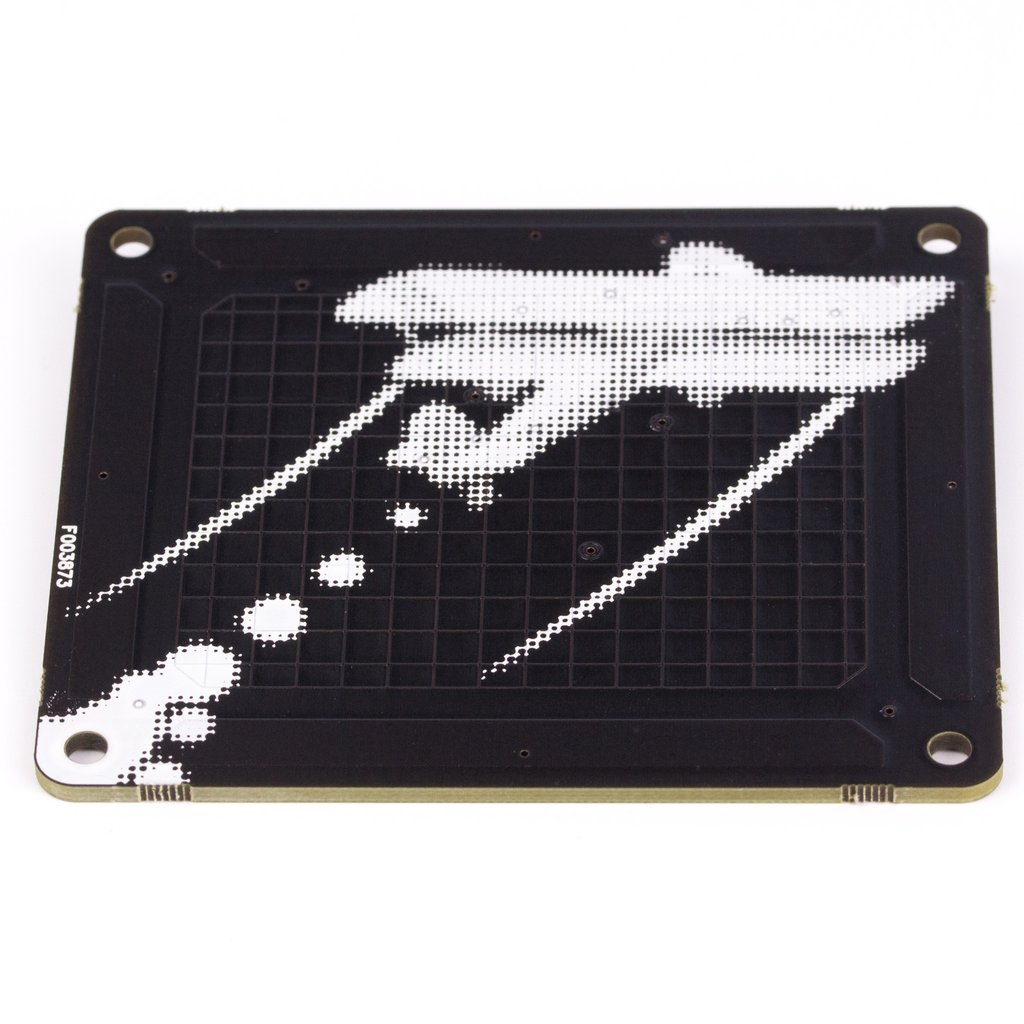
\includegraphics[width=1\textwidth, height=0.6\textheight]{skywriter}
    \caption{Touch Board Skydriver by Piromoni}
    \label{fig:TouchBoard}
\end{figure}
